\title{Supplementary Material for the article `The Beauty Contest On Amazon Mechanical Turk: Going Further Into The Field'}
%\maketitle

\section{Materials and Method}
Amazon Mechanical Turk (MTurk) is an online labor market and crowdsourcing platform, which is increasingly being used for social and economic experiments in order to investigate the real time interactions of small to medium sized groups. MTurk has repeatedly been shown to meet or exceed the standards set by data collection methods using other means \citep{berinsky_huber_lenz_2012, BuhrmesterEtAl18}. The platform has a large participant pool (called participants), various demographic and quality selection options for researchers, and provides an integrated participant compensation system.

\section{Experimental Design}
After participants accept our ‘HIT’ (‘human intelligence task’), they have to provide informed consent, see Figure \ref{Fig S1}. Then they wait until there are enough participants who have accepted the HIT to form random groups (grouped by arrival) of size 2, 4 or 8, respectively, depending on the treatment condition. When group has been formed, instructions are displayed for 90 seconds, see Figure \ref{Fig S2}. After pressing NEXT, participants see a page where they have to enter into a form field an integer number between 0 and 100. When all participants in a group have done so, a result page is displayed, see Figure \ref{Fig S3}, where they can see their own guess, the guesses of the other players, the average and the 2/3 of the average as well as information about whether they have won a bonus in the current found and what their total payoff is for the time being. After this, the previous steps are repeated for a total of 8 rounds. Every time participants enter a new number, they can see a list of the 2/3 of the average of the previous rounds as shown in Figure \ref{Fig S4}. participants have 90 seconds to think about a number. After eight rounds, participants are required to give feedback by answering the question: ‘What strategy did you use while playing this game?’, after which they are thanked for their participation.

\begin{figure}
\includegraphics[width=1\textwidth]{../images/FigA1.png}\caption{Screen dump of the consent page shown to all participants.}
\label{Fig S1}
\end{figure}

\begin{figure}
\includegraphics[width=1\textwidth]{../images/FigA2.png}\caption{Screen dump of an instruction page for a game with four players.}
\label{Fig S2}
\end{figure}

\begin{figure}
\includegraphics[width=1\textwidth]{../images/FigA3.png}\caption{Screen dump of a result page from a game with four players.}
\label{Fig S3}
\end{figure}

\begin{figure}
\includegraphics[width=1\textwidth]{../images/FigA4.png}\caption{Screen dump of a choice page from a game with four players.}
\label{Fig S4}
\end{figure}

\section{MTurk Setting}
When working with MTurk it is important to consider the right settings in order to get the best data quality possible \citep{ChandlerShapiro16}. Fair wage, attrition rates, removal of duplicate participants and informative feedback are some of the most important issues to address.

Average wage for participants in our experiments was approximately \$15 per hour, which is considered generous according to MTurk guidelines and certainly above the estimated average of \$6 per hour when excluding un-submitted and rejected work \citep{HaraEtAl18}. 

Quitting a study before completing it is prevalent on MTurk, and varies systemically across experimental conditions. Our overall attrition rate was 24\%, which is considered normal \citep{ZhouFishbach16}. The main reason, we believe, was either a player not being able to enter a number within the allotted time, or – more likely – due to a player not bothering to wait for the others to make their guess and therefore quitting prematurely. This was very detrimental for the rest of the group and for the experiment as such, because it meant that the rest of the group would continue the game with one player less, making the whole process much slower and skewing the results. If somebody had quit, we still let the other players finish their game and paid them for their efforts, but we decided to remove those groups from the data analysis. Out of a total of 114 initial groups, 27 groups were thus removed from the final data set, giving an overall attrition rate of 24\%.

All participants automatically received a unique qualification when accepting a HIT, ensuring that they could not play the game twice. In addition, we set the qualification that participants should have completed at least 50 HITs and have an accepted HIT rate of 90\% or above. This is slightly below what is considered to be a good cut off (normally researchers recomment above several hundred completed HITs and an acceptance rate of 96\%), but we decided to give less experiences players a chance in order to not be too selective of participant experience, but 90\% still ensured that we would get somewhat experienced and qualified participants. During our experiments, participants had easy access to our email for questions and possible bug reports. 

\section{Code and Software}
All experiments are coded in the experimental software oTree 1.4.39 \citep{ChenSchongerWickens16} which is based on Python and Django. The code for the data analysis done is available on Github at https://github.com/gavstrik/game-of-regret.

\section{Data Collection and Distribution}
After removing defunct groups, we obtained a total of 2368 guesses from 296 unique participants who played the classic iterated beauty contest game in 50 groups of size 2, 23 groups of size 4, and 13 groups of size 8.

\begin{figure}
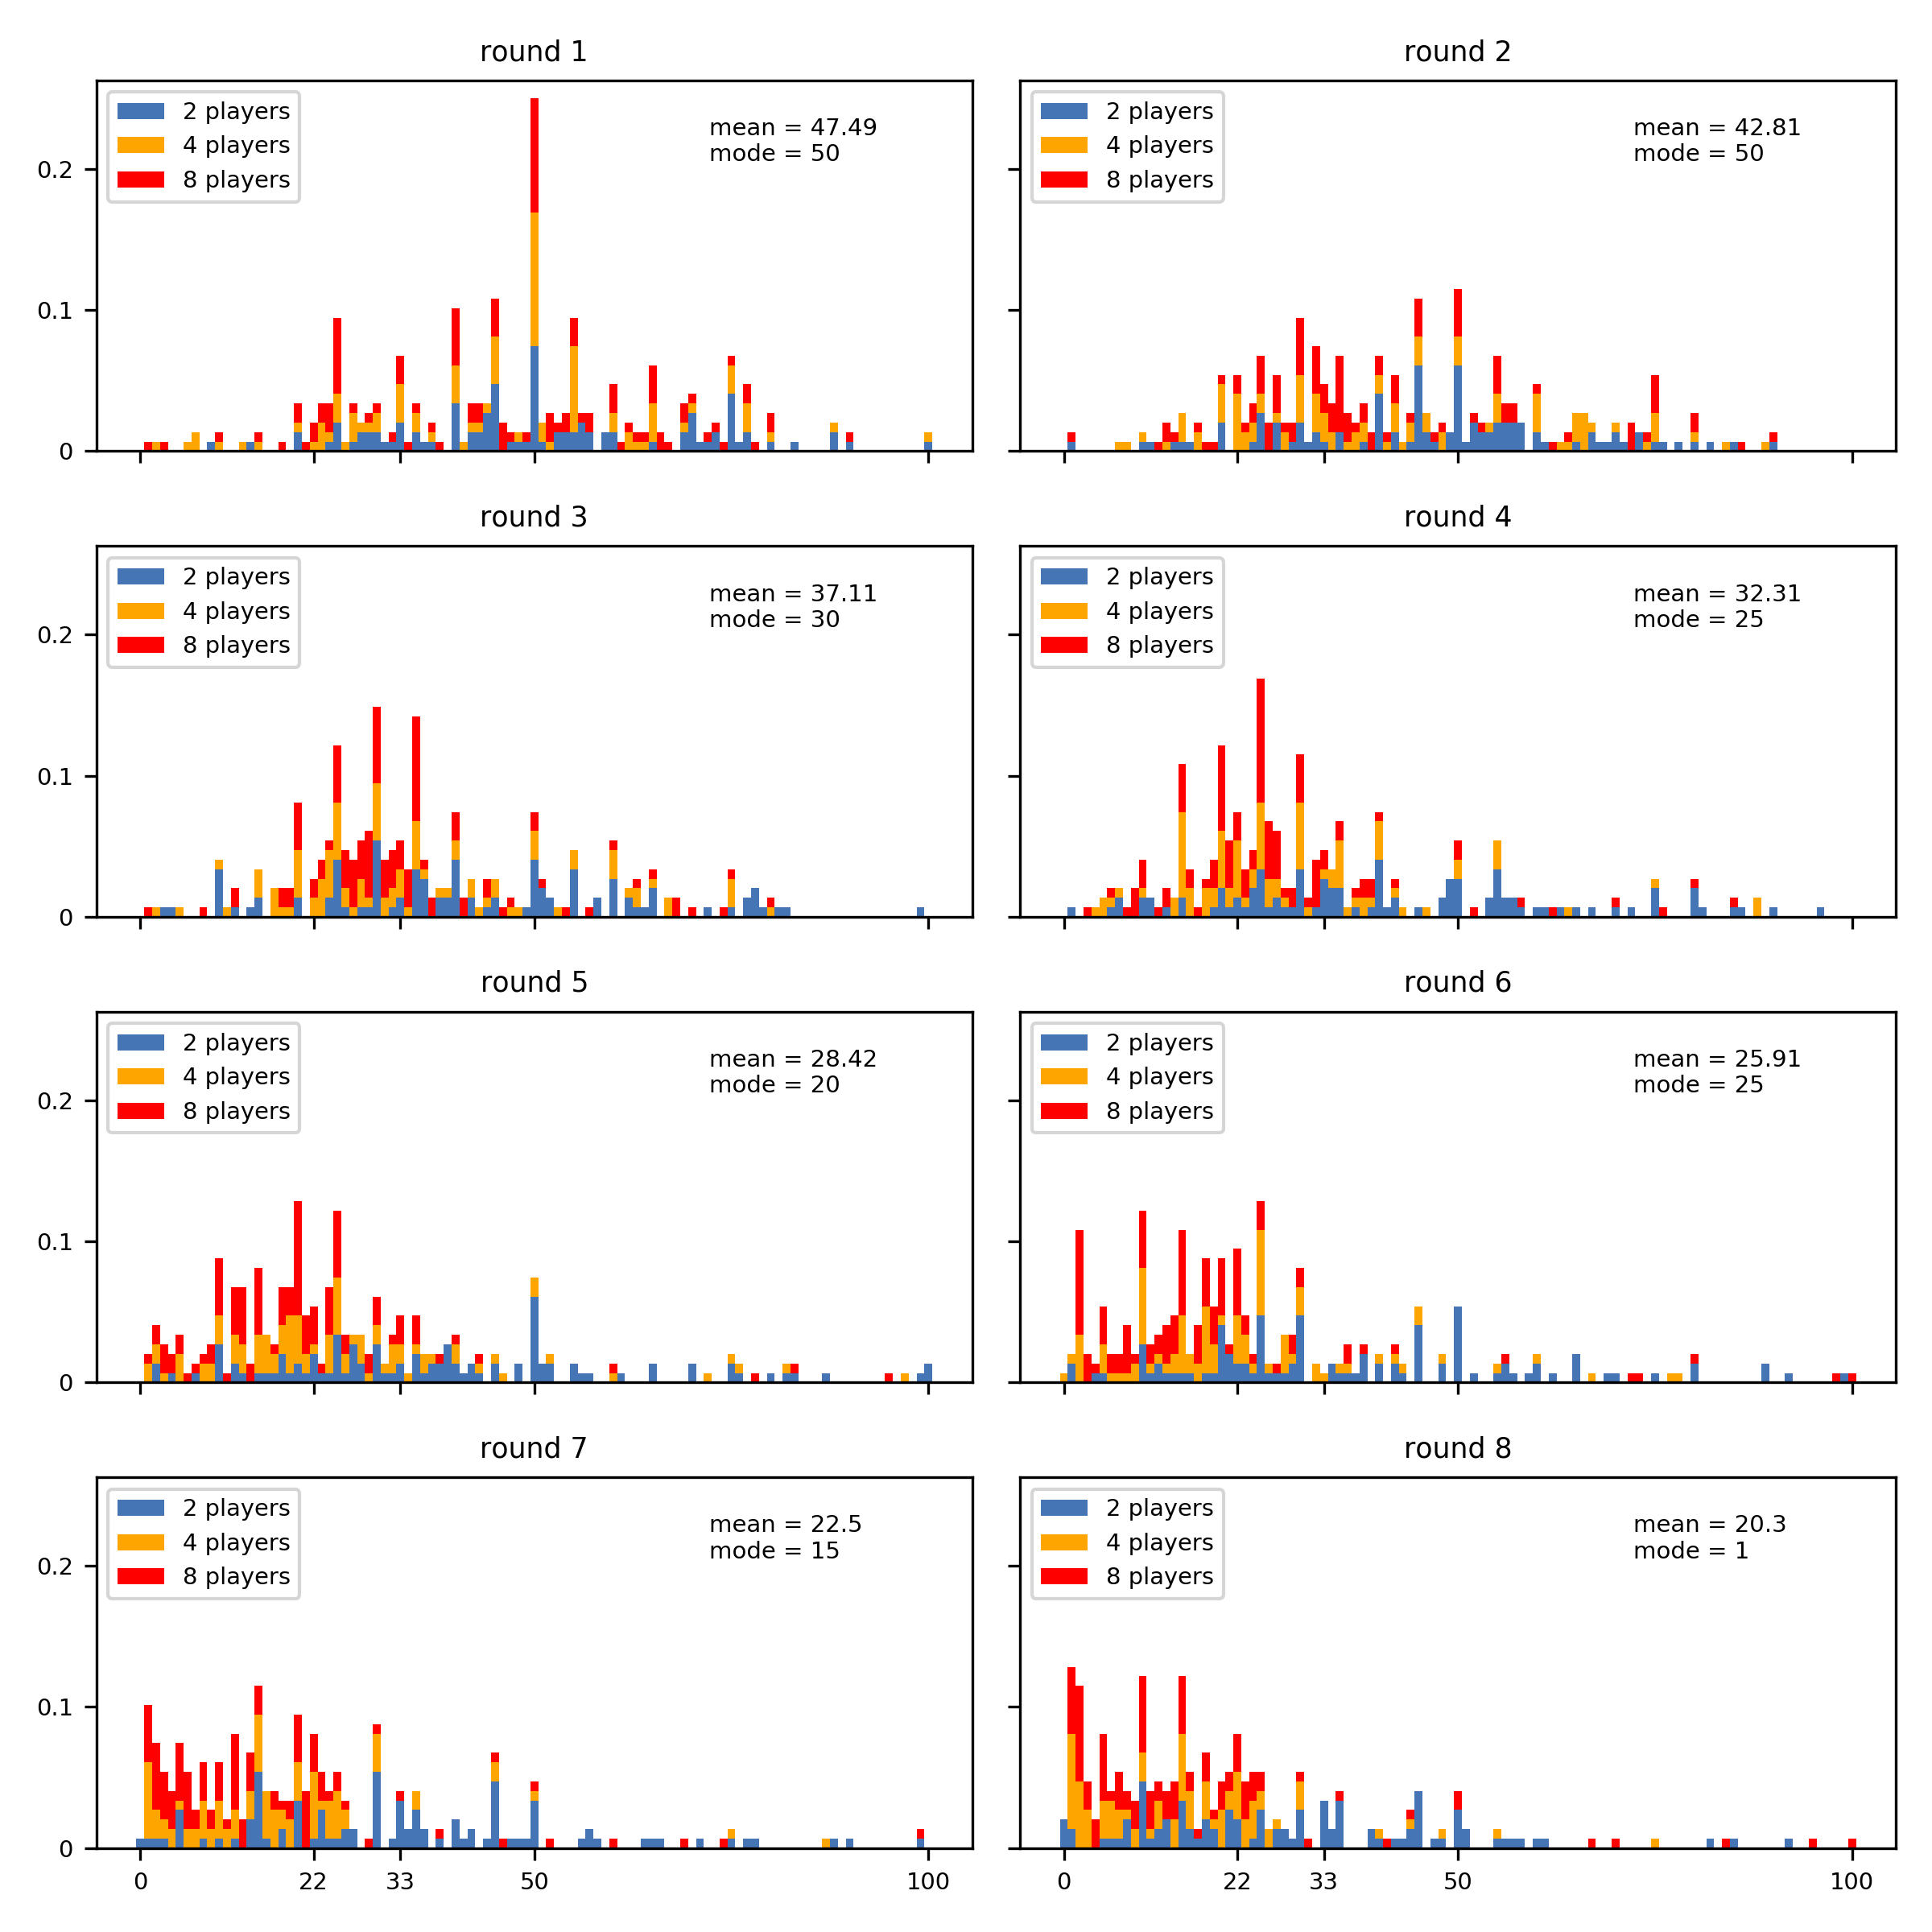
\includegraphics[width=1\textwidth]{../plots/figA5.pdf}\caption{Histograms of guess distributions partitioned into groups and rounds.}
\label{Fig S5}
\end{figure}

Figure \ref{Fig S5} shows the guesses for all eight rounds, partitioned into their respective groups. As can be seen from the histograms, guesses move slowly towards lower numbers in subsequent rounds, with the 2-players groups (in blue) lacking slightly behind the other groups. There are many spikes in the plots, but there is no discernable pattern that would suggest dominant spikes at those positions corresponding to iterated best response strategies (33, 22, etc...).

\section{Guess Dynamics}
As noted in figure 4 in the main text, players often choose numbers greater than 2/3 of the mean of the previous round. Less than 2\% of all players on MTurk never go above 2/3 of the previous mean, while 53\% go above this target more than four times. 

%Figure \ref{Fig S6} shows some examples of the up and down movements of individual guesses from one round to the next. It is difficult to interpret this behavior observed in Fig. S6 as simple directional learning. Instead, players seem to try to “talk” with each other with occasional high guesses, and instead of adapting to the new target (explicitly shown as 2/3 of the previous mean), they may adapt to what they think the other players will guess in the next round.
%
%\begin{figure}
%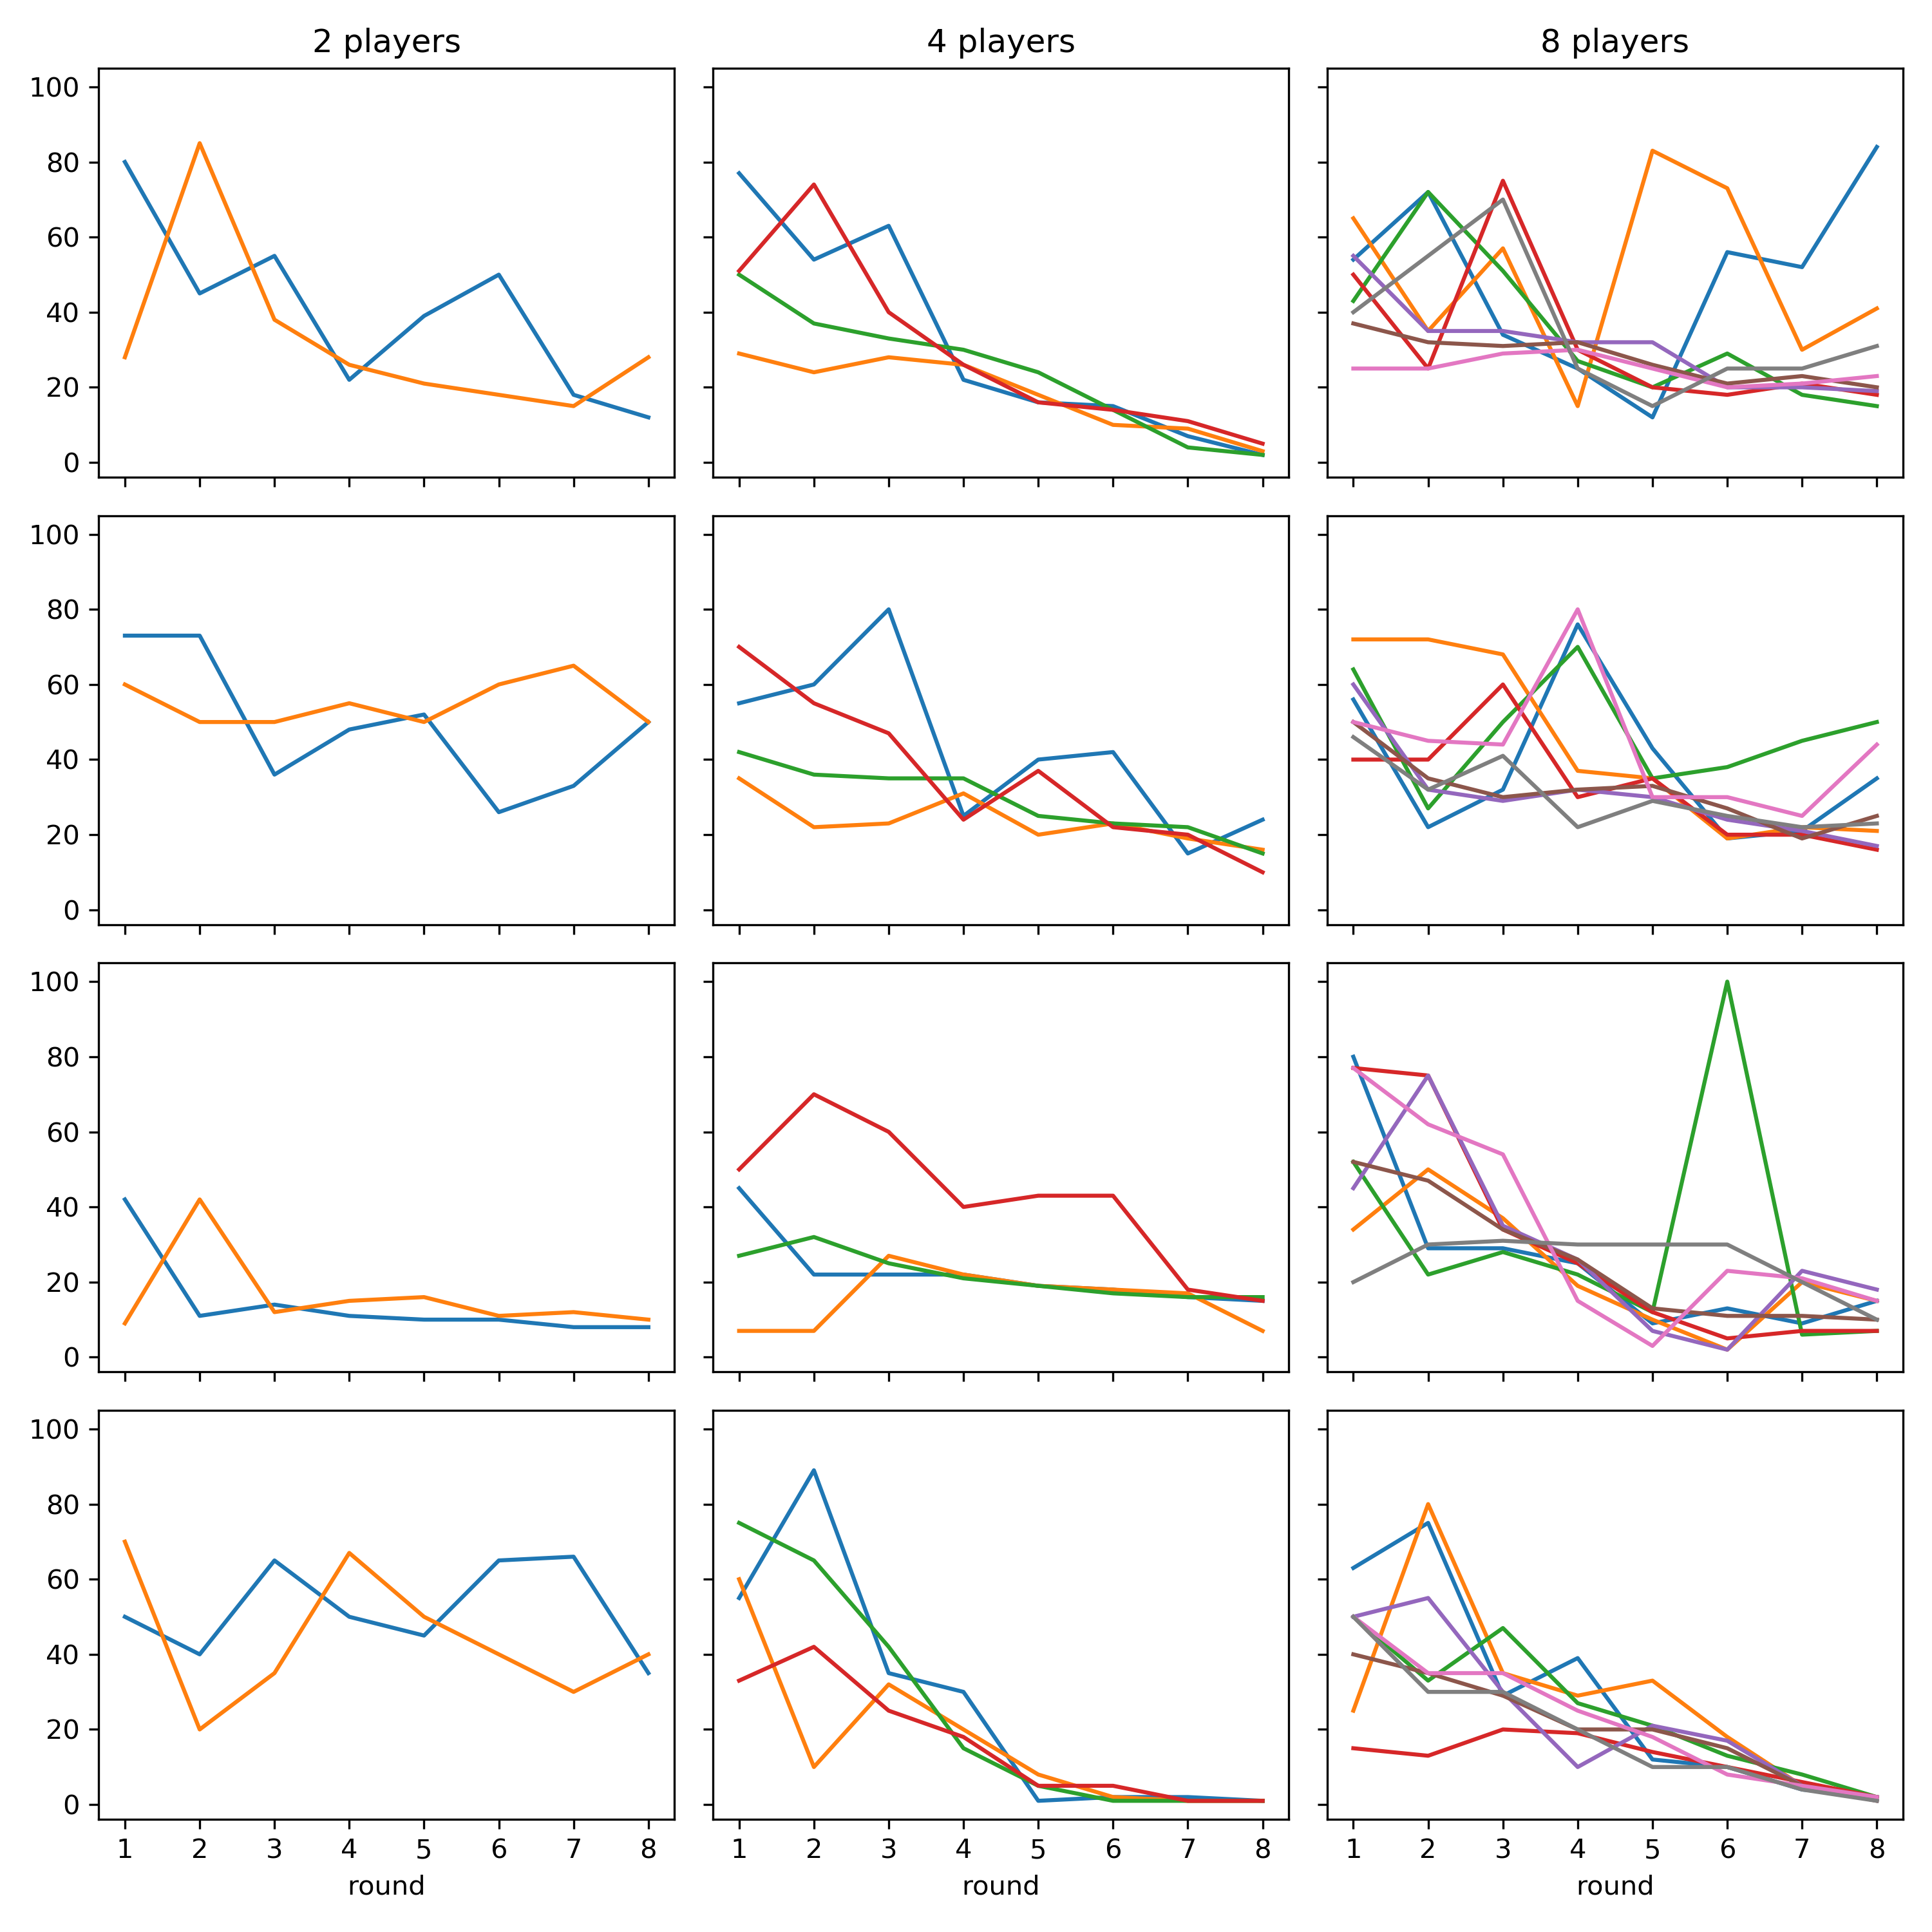
\includegraphics[width=1\textwidth]{../plots/figA6.pdf}\caption{Guess dynamics of player guesses from randomly selected groups.}
%\label{Fig S6}
%\end{figure}
%
%We can illustrate the guess-dynamics in another way as well. 
Figure \ref{Fig S7} shows the dynamics of guesses round by round in such a way that the previous round n is always shown on the x-axis and the next round $n+1$ is always shown on the y-axis. The diagonal black line corresponds to staying at the same guess in subsequent rounds. Lines connecting the dots in Figure \ref{Fig S7} then indicate the sequence of guesses by the same player, whose comments are shown in the legend. The total bonus earned is shown in parenthesis.

\begin{figure}
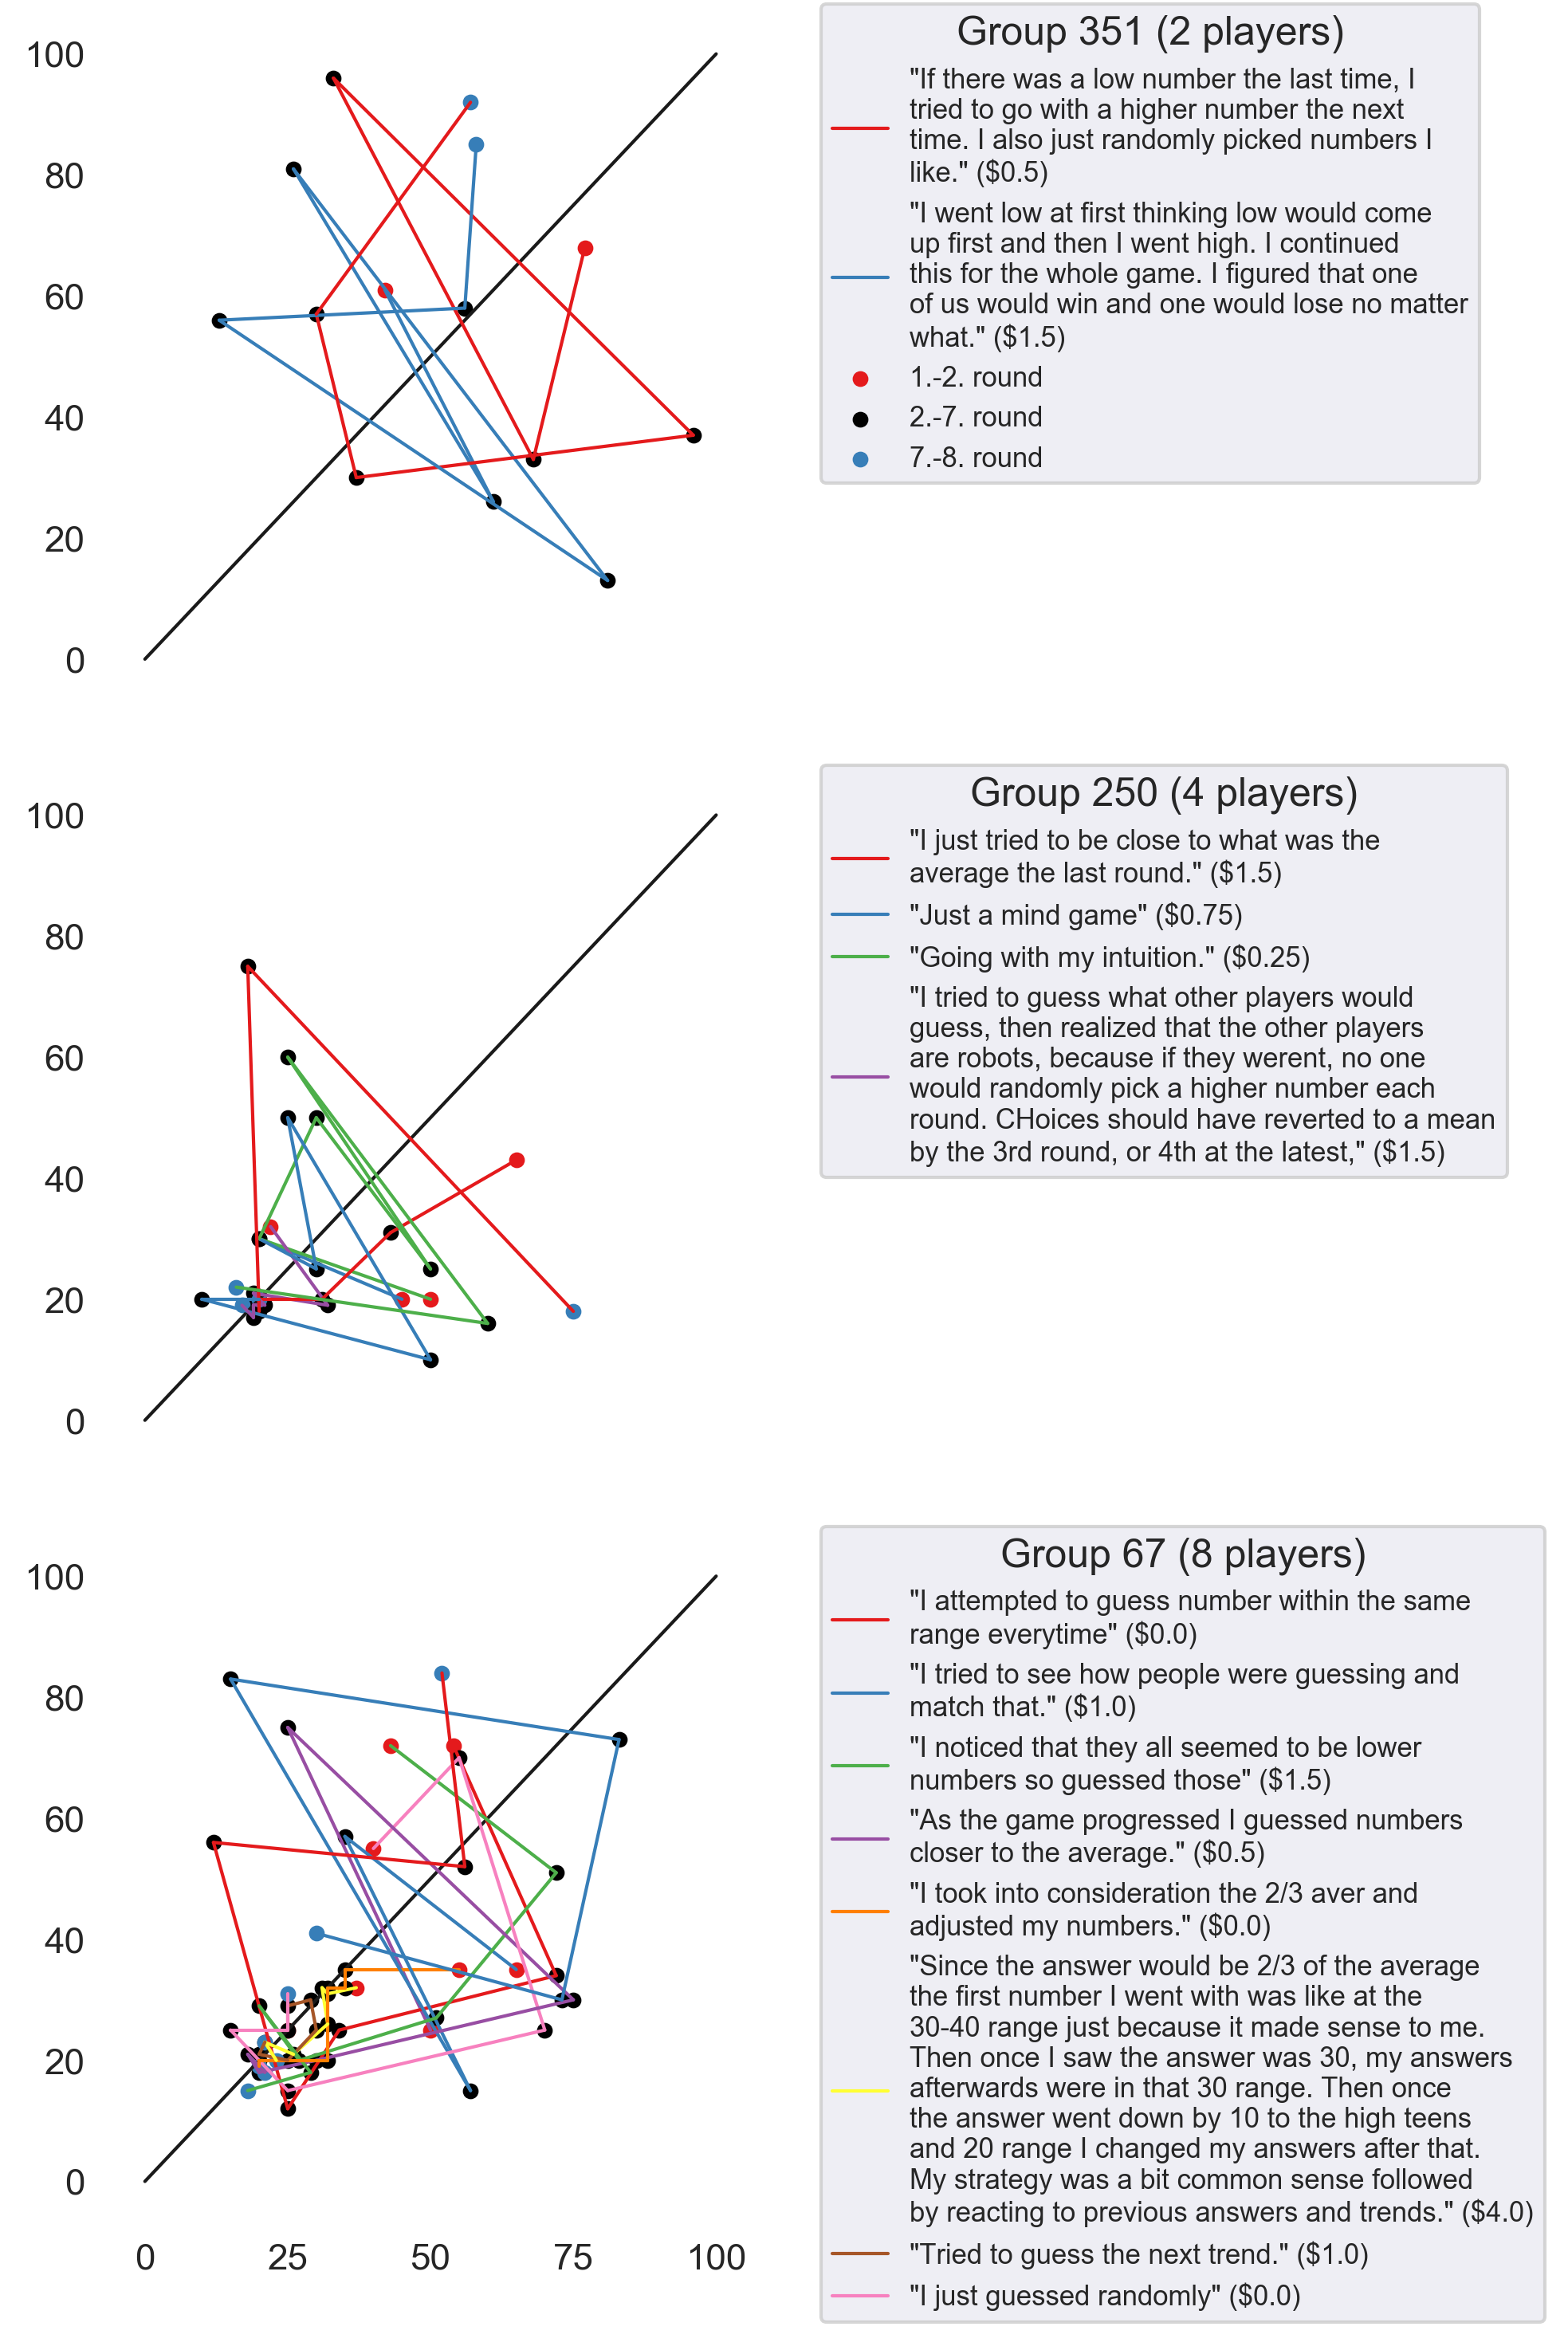
\includegraphics[width=1\textwidth]{../plots/figA7.pdf}\caption{Dynamics of guesses round by round.}
\label{Fig S7}
\end{figure}

\section{Learning rates}
Before fitting a linear regression model to the averages of our groups from MTurk, which will give us an idea of the learning rates of the groups, we need to make sure that the data can be modelled into a Gaussian framework.\footnote{We find that the Nagel data \cite{Nagel95} is not easily fitted in a Gaussian framework. We have tried both the raw average and the log (corresponding to a log-normal model). Therefore we only used the raw averages without confidence intervals in figure \ref{fig:means}.} Looking at the raw avarages for all eight rounds in figure \ref{fig:means} we see some non-linear relationships in the last rounds. To model the averages as a function of group size we therefore use a gaussian general linear model (GLM) \cite{Rcoreteam} with a quadratic interaction term:

\begin{align*}
Y_{ij} &\sim Gaussian(\mu_{ij}) \\
\mathbf{E}(Y_{ij}) &= \mu_{ij}  = g^{-1}(X\beta) \\
g(\mu_{ij}) &= (round + round^2) \, \times \, size \\
\alpha &\sim \mathcal{N}(\mu,\,\sigma^{2})\,.
\end{align*}

where $Y_i$ are the averages for each round $i \in {1,..., 8}$  and each group $j \in {2,4,8}$
$\alpha_i$ is the random intercept, which is assumed to be normally distributed with mean $0$ and variance $\sigma^2$. 


To validate the model we plot its standardized residuals against the theoretical quartiles in figure \ref{fig:qq}, which show a very good fit with normally distributed residuals. Tails are obviously not captured all that well, but this is not to be expected. Besided, the linear regression model is quite robust to some degree of deviation from the assumption of normally distributed residuals. In addition, the majority in the middle values are captured near perfectly, hence we cannot reasonably discard the linear regression model.

\begin{figure}
\includegraphics[width=1\textwidth]{../plots/qq.pdf}\caption{QQ plot showing normally distributed standardized residuals.}
\label{fig:qq}
\end{figure}


